\section{Оборудование и инструментальные погрешности}

\subsection{Балиистический маятник, совершающий поступательное движение}

Баллистический маятник представляет собой тяжёлый цилиндр, подвешенный на четырёх
нитях одинаковой длины. При колебаниях такой маятник совершает поступательное
движение.

\begin{figure}[ht!]
    \centering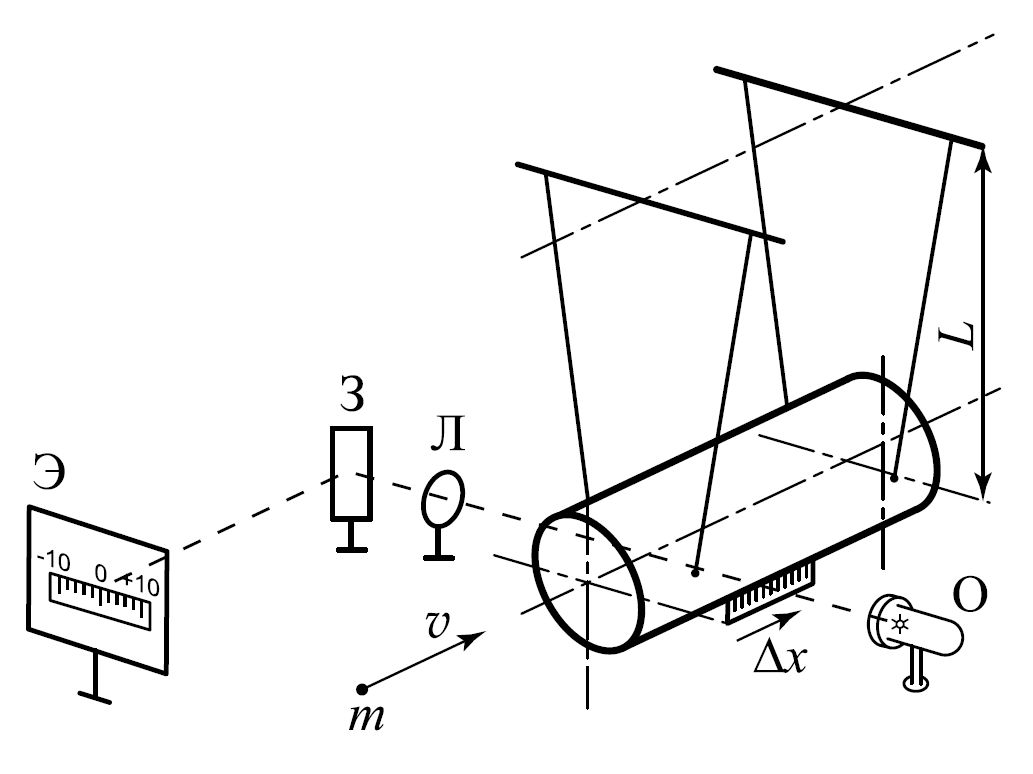
\includegraphics[width=0.8\linewidth]{img/scheme1.png}
\end{figure}

Скорость пули при ударе должна быть направлена вдоль оси цилиндра.

\begin{figure}[ht!]
    \centering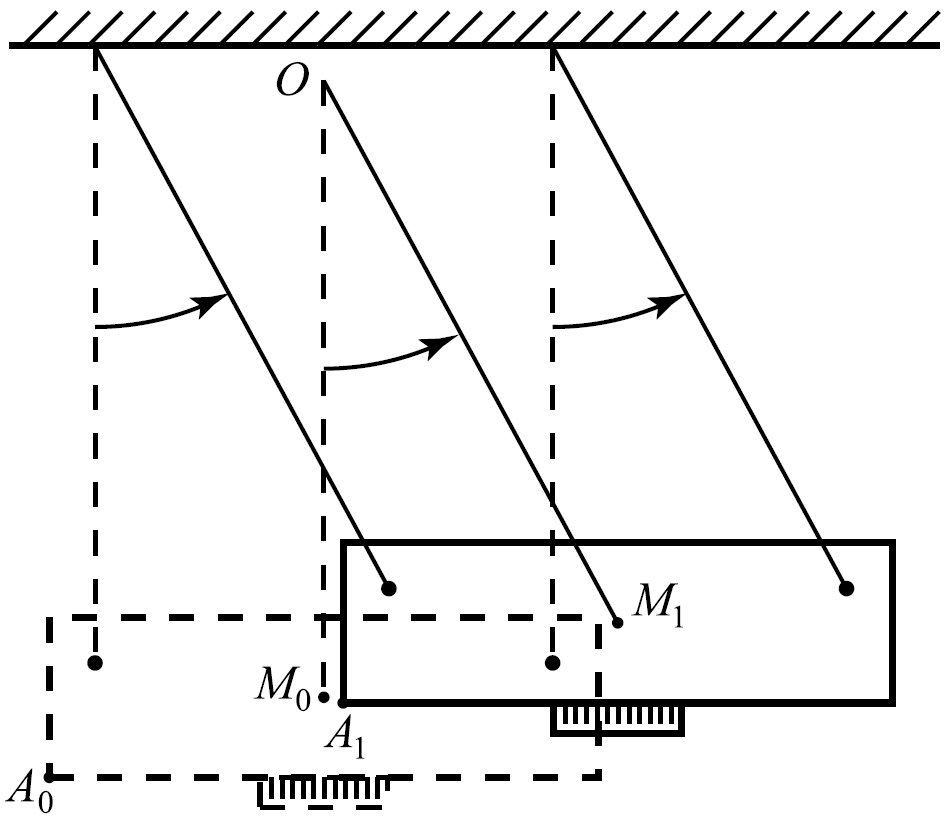
\includegraphics[width=0.8\linewidth]{img/scheme2.png}
\end{figure}

Закон созранения импульса
\[mu=\left(M+m\right)V\]
$m$~--- масса пули, $M$~--- масса цилиндра, $u$~--- скорость пулидо удара, $V$~---
скорость пули после удара.

Т.к. масса маятника значительно превышает массу пули
\[u=\frac{m}{M}V\]

Из закона сохранения энергии получим связь с максимальной высотой подъёма $h$:
\[V^2=2gh\]
Связь максимальной высоты со смещением по горизонтали $\Delta x$:
\[h=2L\sin^2\frac{\Delta x}{2L}\]

Итого:
\[u=\frac{M}{m}\sqrt{\frac{g}{L}}\Delta x\]

$\Delta x$ определяется при помощи оптической системы. Затухание можно назвать слабым,
если за 10 периодов амплитуда уменьшается не более, чем вдвое.

\subsection{Крутильный балиистический маятник}
\begin{figure}[ht!]
    \centering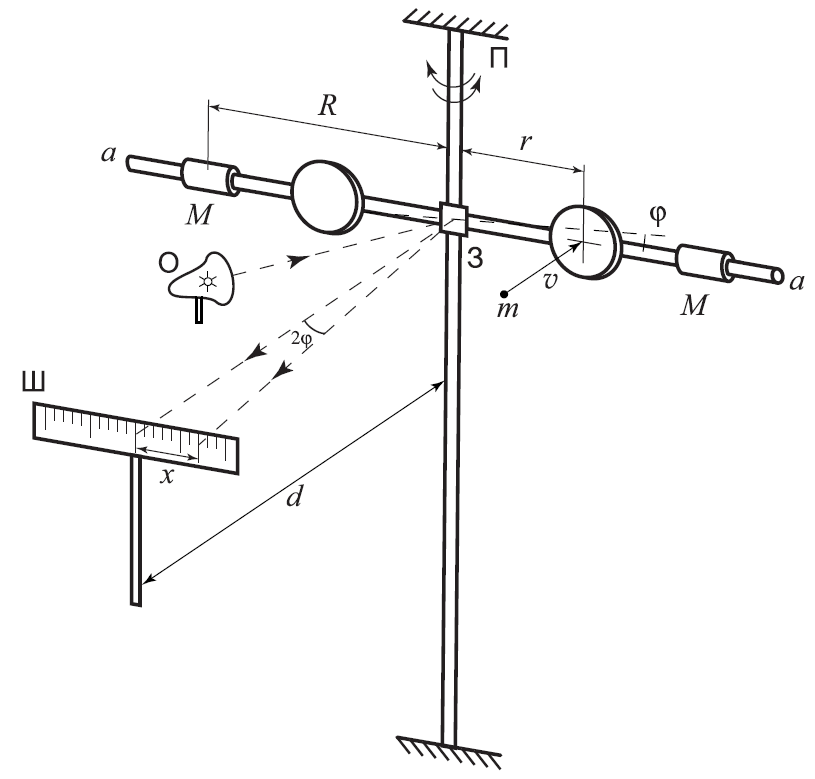
\includegraphics[width=0.8\linewidth]{img/scheme3.png}
\end{figure}

Пуля массой $m$ попадает в мишень, укреплённую на стержне $aa$, который образует
крутильный маятник с грузами $M$ и проволокой $\Pi$.

Из закона сохранения момента импульса
\[mur = I\Omega\]
$r$~--- расстяоние от линии пролёта пули до оси вращения маятника, $I$~--- момент инерции
маятника, $\Omega$~--- его угловая скорость сразу после удара.

Время соударения должно быть много меньше периода. Произведение момента кручения в момент
соударения на время соударения мало по сравнению с моментом импульса пули. Закон сохранения
энергии:
\[k\frac{\varphi^2}{2}=I\frac{\Omega^2}{2}\]
$k$~--- модуль кручения проволоки, $\varphi$~--- максимальный угол поворота.

\[u=\varphi\frac{\sqrt{kI}}{mr}\]
\[\varphi\approx\frac{x}{2d}\]
$x$~--- смещение изображения нити, $d$~--- расстояние от шкала до оси вращения маятника.

$kI$ можно найти из соотношения периодов колебания маятника с грузами и без них:
\begin{gather*}
    T_1=2\pi\sqrt{\frac{I}{l}}\\
    T_2=2\pi\sqrt{\frac{I-2MR^2}{k}}\\
    \sqrt{kI} = \frac{4\pi MR^2T_1}{T_1^2-T_2^2}\\
\end{gather*}
$R$~--- расстояние от центров масс грузов $M$ до проволоки.
